\chapter{Architecture}
This chapter discusses the changes made to the internal architecture of the application. While most of those changes were motivated by some technical need or issue, we also made changes so that it is possible to use a properly secured connection which helps us further protect the privacy of our users and the security of their data. The details about those change are explained in details in section \ref{sec:proxy} and in particular the subsection \ref{subsec:privacy} is aimed at explaining the implications and benefits on our users' privacy and security.
\section{Previous architecture}
The previous architecture has at its core goal to isolate as much as possible the processes handling our users' private data from the outside world. As can be seen in figure \ref{fig:fetchArch} and figure \ref{fig:gameCreationArch} the Game Creator (also sometimes called Game Generator) process does not accept request from the outside world and everything goes through the Reminisce.me component. This component itself accepts requests from the outside world but never handles the data we get from Facebook, it can only get the created game boards from the Game Creator, never the actual piece of data used to generate it.\\
While this architectures is really good at preventing private data from leaking to a potential malicious user (thanks to the fact that we authenticate our users through Facebook authentification), it does not help the user to verify the identity of the server. This setup is quite vulnerable to what is called a Man-in-the-middle attack\cite{mitm} and the communication is not encrypted. In short, a malicious person could (with more or less ease) intercept messages and read the generated questions (which contain some of the user's Facebook data) by pretending to be the server and simply relaying the messages.
A simple solution to this is the use of SSL\cite{whyssl}.\blockquote{Transport Layer Security (TLS) and its predecessor, Secure Sockets Layer (SSL), both frequently referred to as "SSL", are cryptographic protocols that provide communications security over a computer network.\cite{ssl}}
It works by generating a proof of identity (certificate) via a Certificate Authority\cite{ca} (CA) and sending it to the user when establishing a connection. The browser can then verify the validity of the certificate with the help of the CA. All of these operations are transparent to the end user and come only at a small cost of performance which is unnoticeable for a human user. More about the benefits on privacy is said in section \ref{subsec:privacy}. As a Certificate Authority we chose to use Let's Encrypt\cite{letsencrypt} which is a free certificate authority supported by a lot of renowned corporations.
\begin{figure}[!h]
\center
{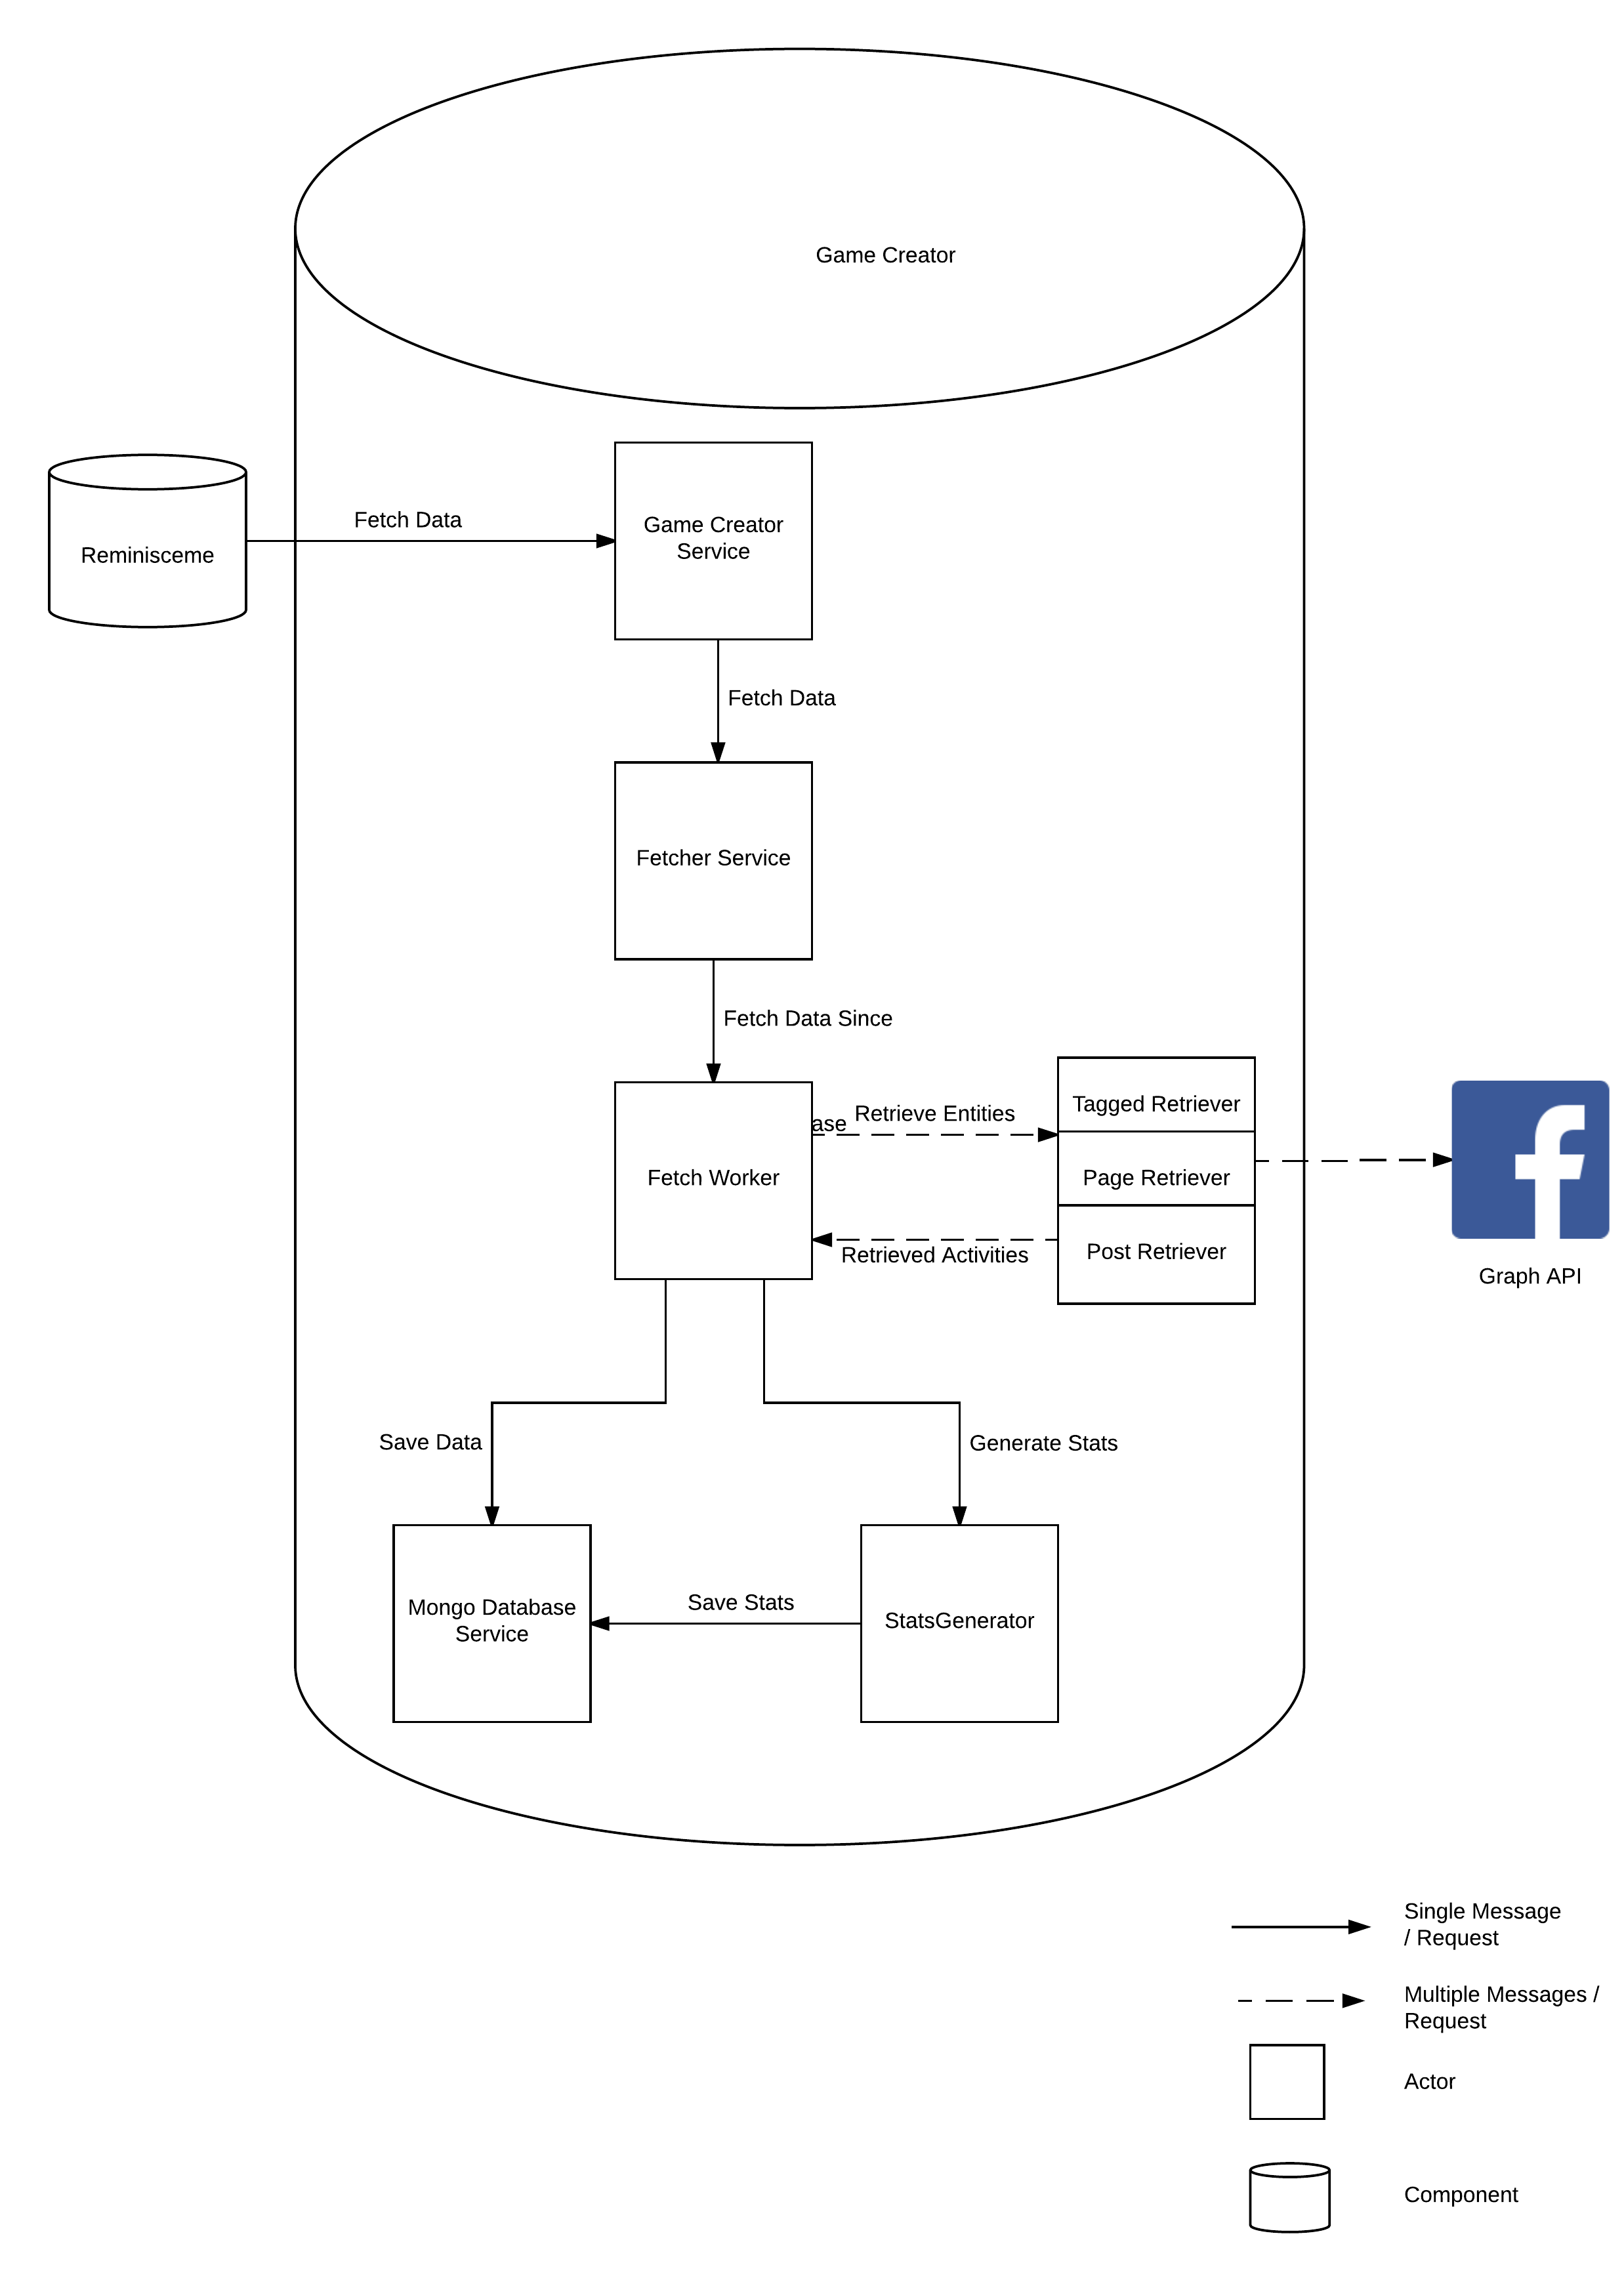
\includegraphics[width=3.5in]{images/fetch_arch.png}}
\caption{Fetching architecture schema}
\label{fig:fetchArch}
\end{figure}
\begin{figure}[!h]
\center
{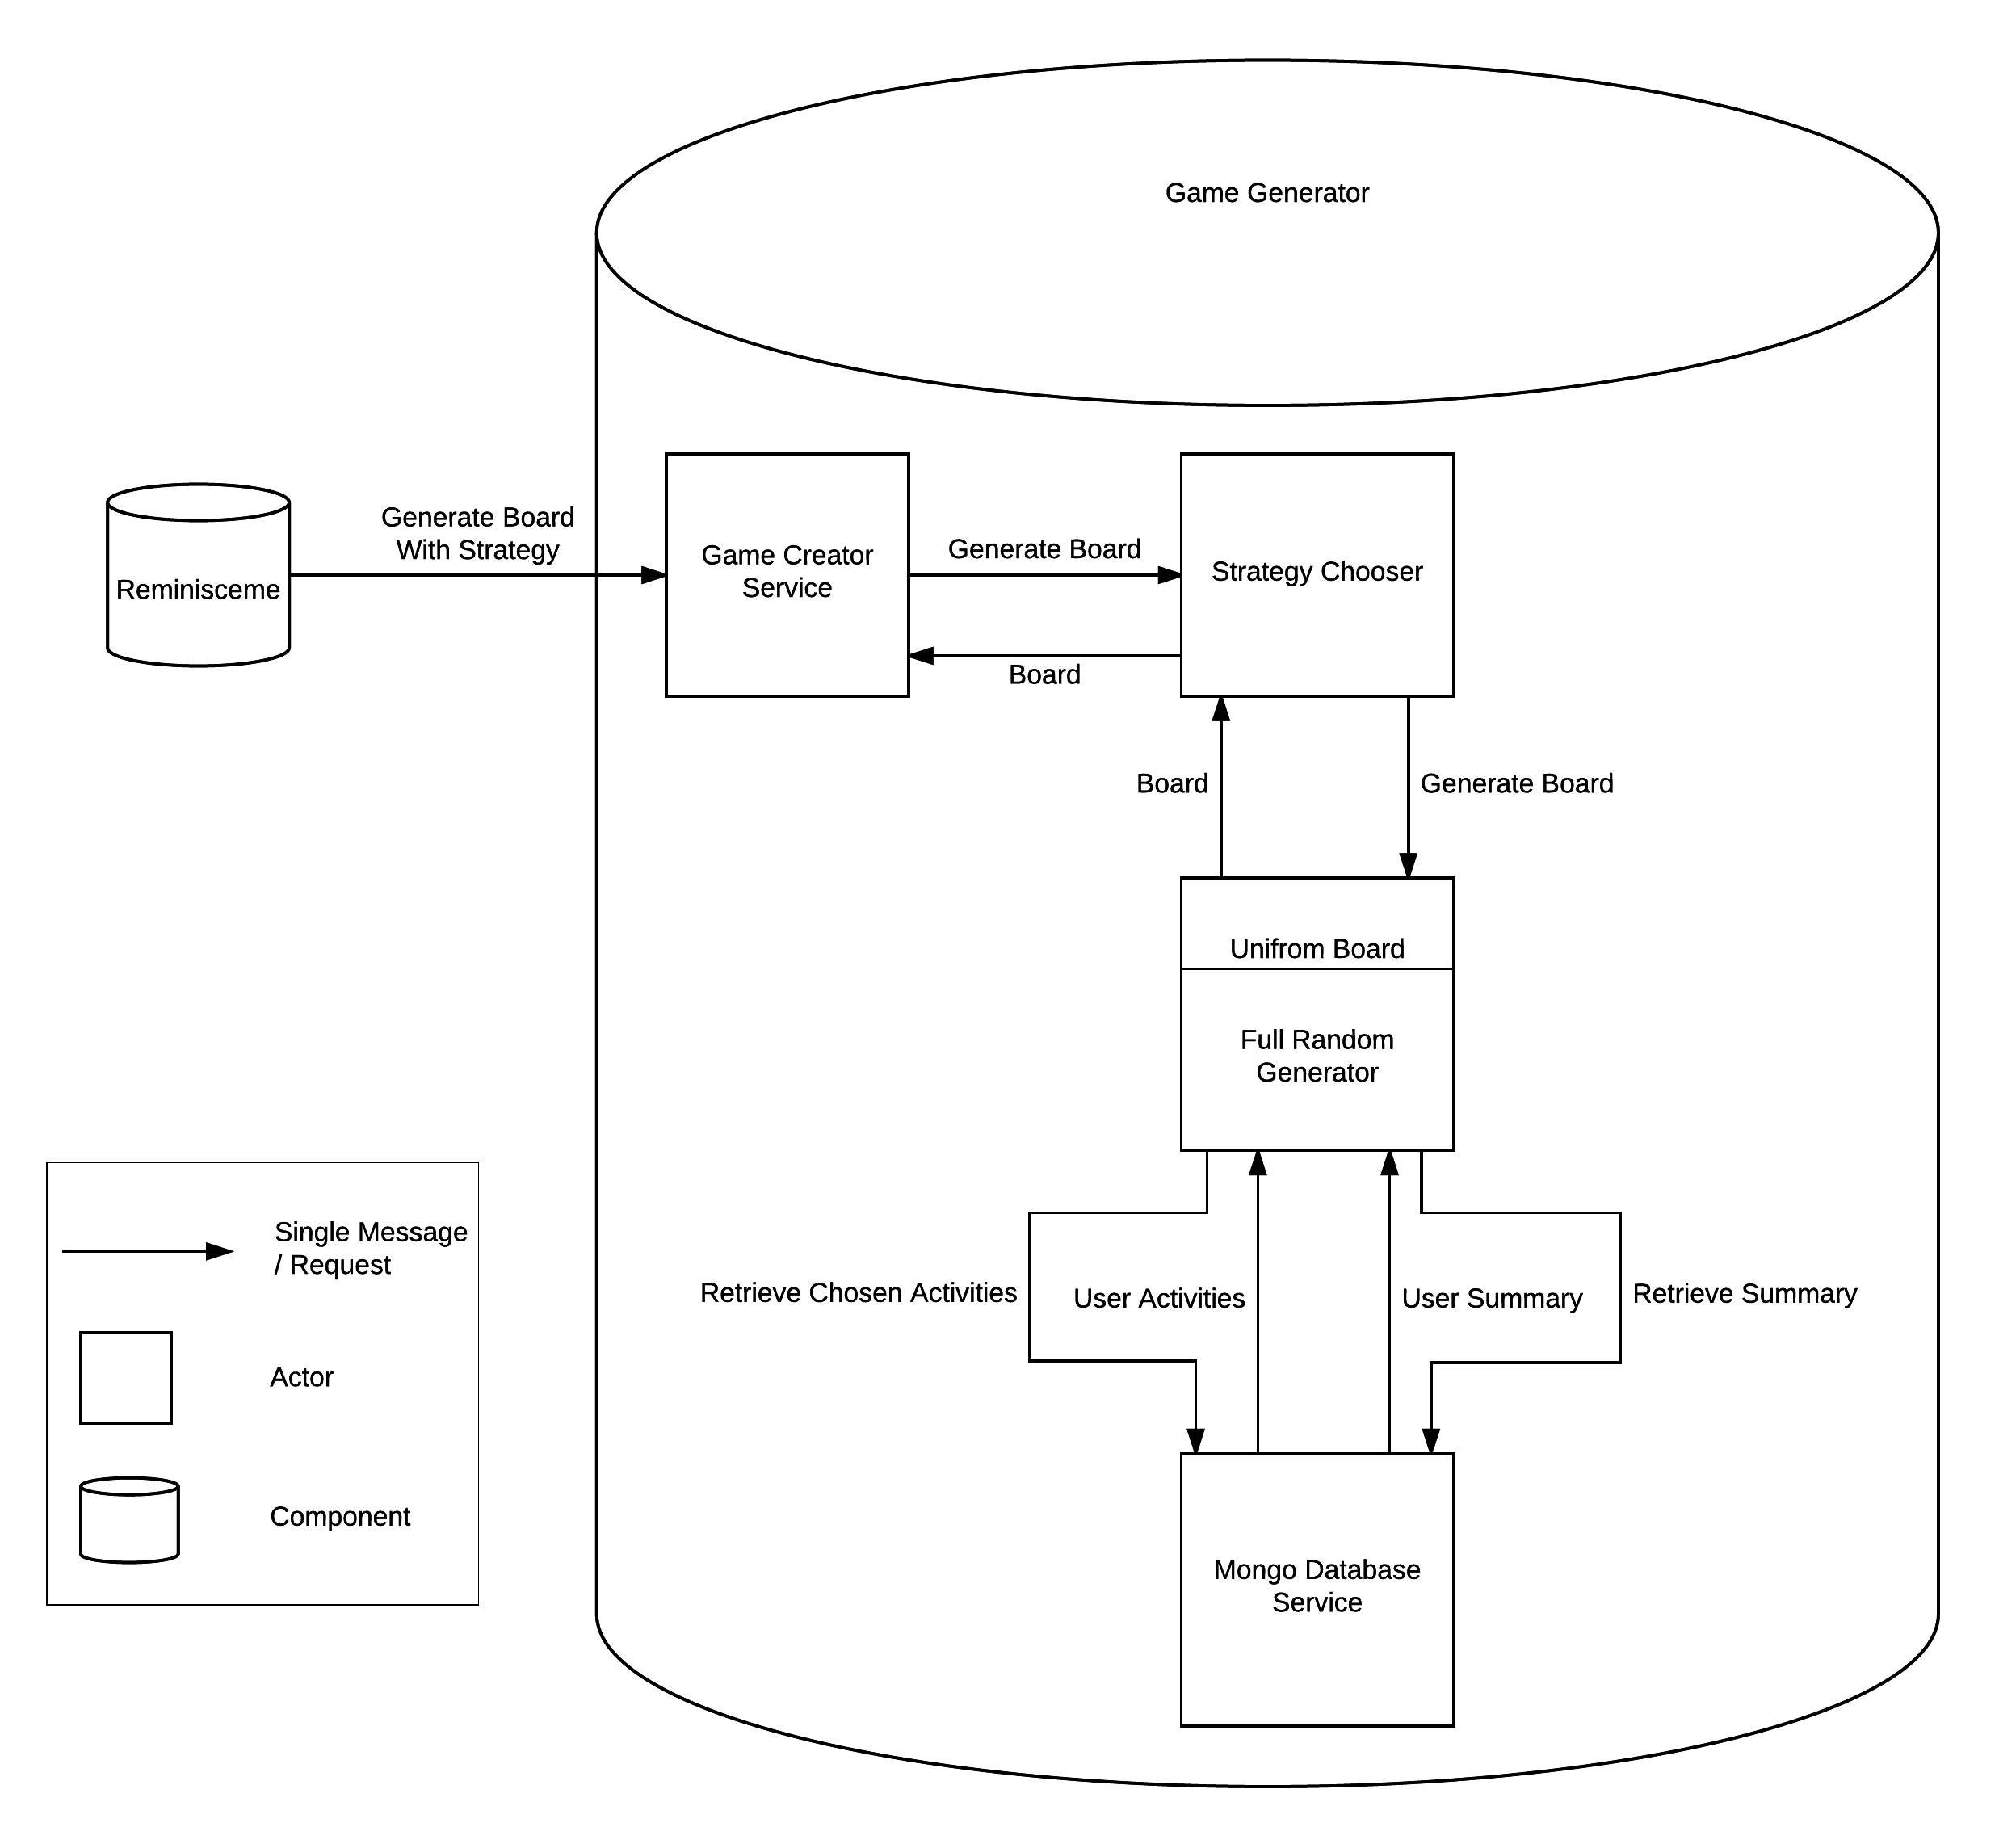
\includegraphics[width=3.5in]{images/gc_arch.png}}
\caption{Game generation schema}
\label{fig:gameCreationArch}
\end{figure}
\section{A proxy to face the world}\label{sec:proxy}
As mentioned earlier, it was crucial for the privacy of our users that we start using some cryptographic protection. Using SSL certificates properly implies doing a lot of sometimes complicated cryptographic work. It is never advised to try and implement this kind of protocol by oneself. In fact it is one of the most common security mistakes\cite{selfcrypto}. This is the first reason we needed to introduce a proxy\cite{reverseproxy}. It is a piece of software that will serve as a single point of communication between the "outside world" and our application. Most of the modern proxies are simply able to use the SSL protocol and serve the requests to our application in a transparent way. Which means that, by simply adding a proxy in font of our application we can add a lot of privacy protection and trust (more in subsection \ref{subsec:privacy}).\\
An other reason we were interested in having a proxy in place is that we wanted to have some administrative tools available easily from the same server as the application (in particular we wanted to be able to easily consult the logs (\ref{sec:logging}) generated by the application if anything went wrong) and a proxy's main function is actually to serve information from multiple processes on a single access point.\\
It can also be seen as "doubling" the isolation of the Game Creator by putting an other layer of protection on top of the previous one, while not necessarily mandatory, it is always a good idea to rely on tested and widespread software rather than our own only when it comes to security.\\
Finally, a proxy would facilitate the transition to a model with multiple machines instead of one if we would need to have more computing power. This is because the modern proxies are equipped with all the necessary tools to perform load-balancing (``load balancing improves the distribution of workloads across multiple computing resources'' \cite{loadbalancing}).
We decided to use NginX\cite{nginx} for the above-mentioned reasons, a lot of people use it (which also means that it is easier to find information about it online), it has been proven reliable and powerful and it supports a lot of useful features such as preventing user to access the server without using the SSL protocol (everything is handled in a transparent way and the user never has to think about it).
\subsection{Privacy and security}\label{subsec:privacy}
To understand the benefits of using a proper SSL certificate and protocol, it is important to understand a bit more about how it works. As mentioned before, it is used mainly to allow the user to identify the server or website as being who it is pretending to be and to allow encryption of the exchanged messages. Any well-configured server using SSL will be able to show a certificate to the user's browser which the latter can verify with the Certificate Authority which produced it. The Certificate Authority will make sure that:
\begin{enumerate}
	\item The certificate is indeed the valid one for the visited website.
	\item The person which originally generated the certificate is the owner of the website which is being certified.
	\item The certificate has not been revoked by its owner
\end{enumerate}
If those conditions are met, the browser will be able to trust the website and the user will have a visual confirmation that this site can be trusted (it usually is a green lock or text in the address bar ads shown in figure \ref{fig:sslBar}). The browser can also now establish a securely encrypted connection with the server preventing anyone from reading the messages exchanged. When the user sees that the website is trusted by the browser, they can trust that their data is handled in a responsible way. As a side note, it is possible to assess the quality of the configuration of a server by using a testing benchmark, for instance, here are the results for the domain \url{reminisce.me} on the Qualys SSL Labs benchmark\cite{ssllabs}: \url{https://www.ssllabs.com/ssltest/analyze.html?d=reminisce.me}.
\begin{figure}
\centering
{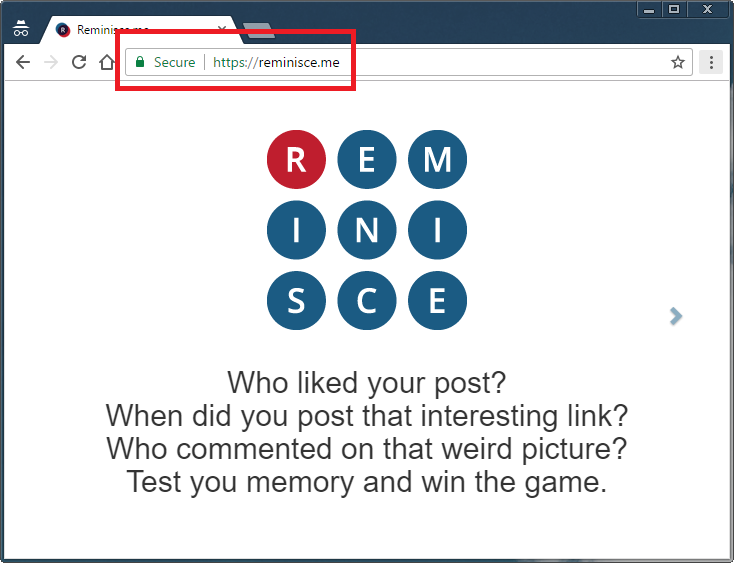
\includegraphics[width=3.5in]{images/ssl_bar.png}}
\caption{Trusted website}
\label{fig:sslBar}
\end{figure}
\section{Monitoring and logging}\label{sec:logging}
When developing and maintaining an application, one of the key feature required to be able to find, understand and eliminate defect, is the ability to understand the failure. One need to be able to see where the failure happened, what the state of the system was and if possible the cause of the failure. In order to achieve this, a well thought logging system is mandatory. This means that the application must produce logs that are readable and explanatory, they must provide as much information as possible so that the cause of failure can be identified rapidly. On top of this, one need to be able to search through the logs in a convenient way, which is not a given because with a large number of user the log can start to grow a lot.\\
One of the common usage of the log is to find why one user encountered the problem which was reported, when this is the case we need to be able to find all actions performed by the application for that user. With this in mind, we made sure that whenever possible an identifier for the user who triggered the action is added to the log.
\subsection{Indexing the log and looking at it}
We wanted to be able to easily answer questions such as "How often does this problem happen?". To be able to do this in the easiest way, we have to provide a search interface which provides tools for searching and analyzing the logs. Fortunately, this is a common issue when building an application so solutions already exist. We decided to use ElasticSearch\cite{elasticsearch} and Logstash\cite{logstash} to index the logs. As shown on figure \ref{fig:loggingArch}, the Game Creator and the application both write their logs to a file, Logstash then reads those files and feeds them into the ElasticSearch database which then makes them easily searchable (by using the Elastic Search Query DSL \cite{querydsl}). Finally we use Kibana\cite{kibana} to have a nice graphical interface to access the indexed logs. It provides ways to formulate queries and generate graphs which can help monitor certain events such as the number of detected failures. Figure \ref{fig:kibana} shows an example of the graphical interface Kibana provides.
\section{Protecting the logs}
Having the logs easily accessible from the website is a really useful feature and it can prove really helpful. But it is also a privacy risk. We want the logs to be as informative as possible and therefore they may contain pieces of information we do not want to be leaked to the general public. For that reason it is necessary to use some sort of authentication scheme. To make it transparent and avoid having to handle a user system (or have a password that we have to change whenever anyone leaves the team) we simply decided to use the information we get from Facebook, which contains the role of a user in the application (simple user or developer). We then use HTTP cookies to tell NginX that this user is trusted. \blockquote{An HTTP cookie (also called web cookie, Internet cookie, browser cookie or simply cookie) is a small piece of data sent from a website and stored on the user's computer by the user's web browser while the user is browsing.}\cite{cookie} After being stored on the user's web browser, these cookies will be sent with all the requests made to the website and the proxy can then read them and make sure the user is an authorized user. We made sure that they are encrypted so that no one can steal them and use them to look at the logs. Appendix \ref{appendix:cookies} explains in more details how this was achieved.
\begin{figure}
\centering
{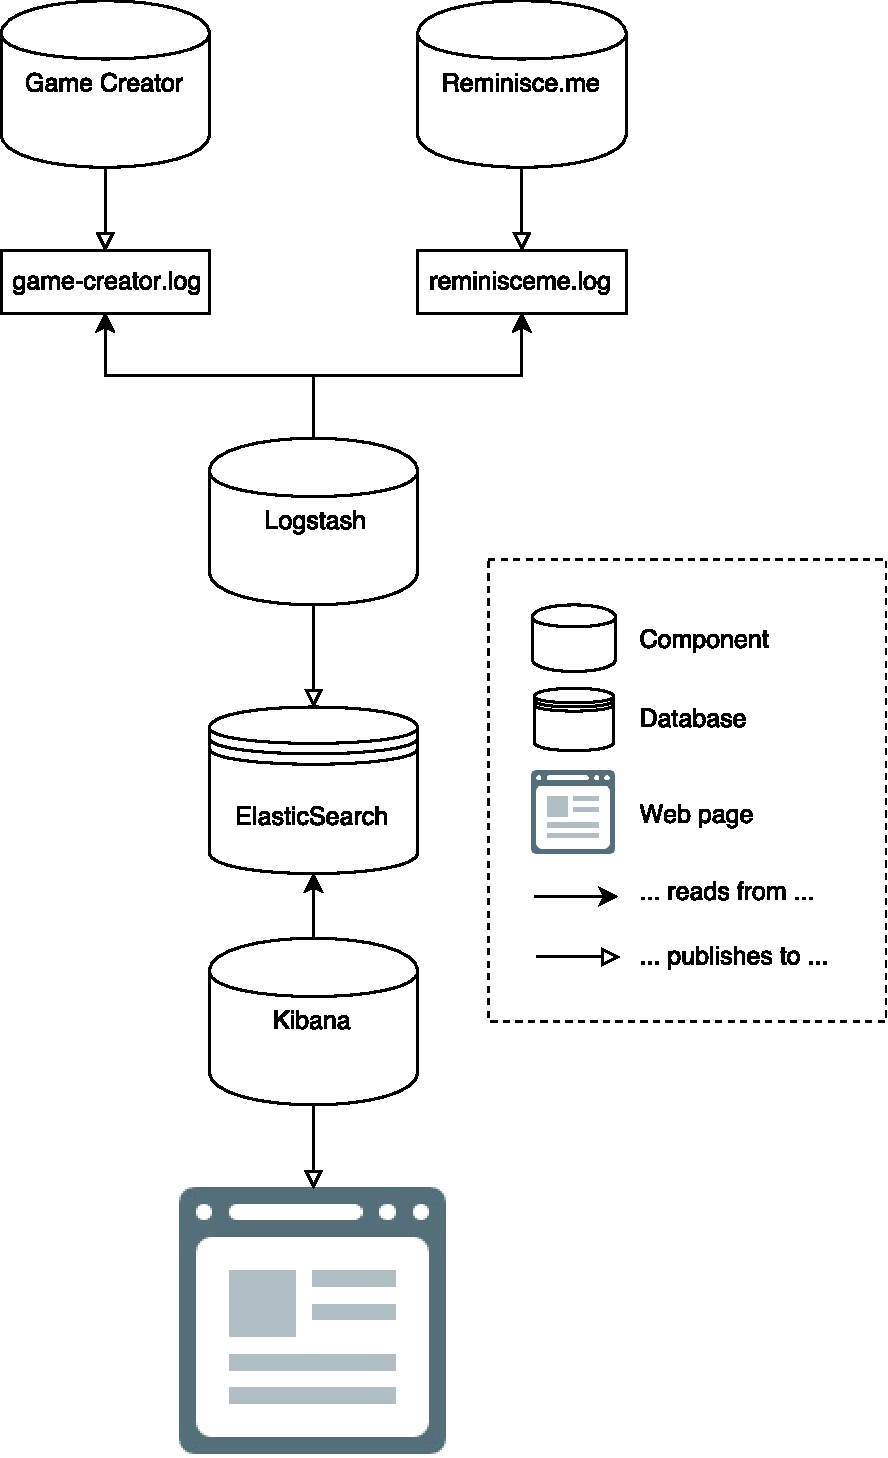
\includegraphics[width=3.5in]{images/logging_arch.pdf}}
\caption{Logging architecture}
\label{fig:loggingArch}
\end{figure}

\begin{figure}
\centering
{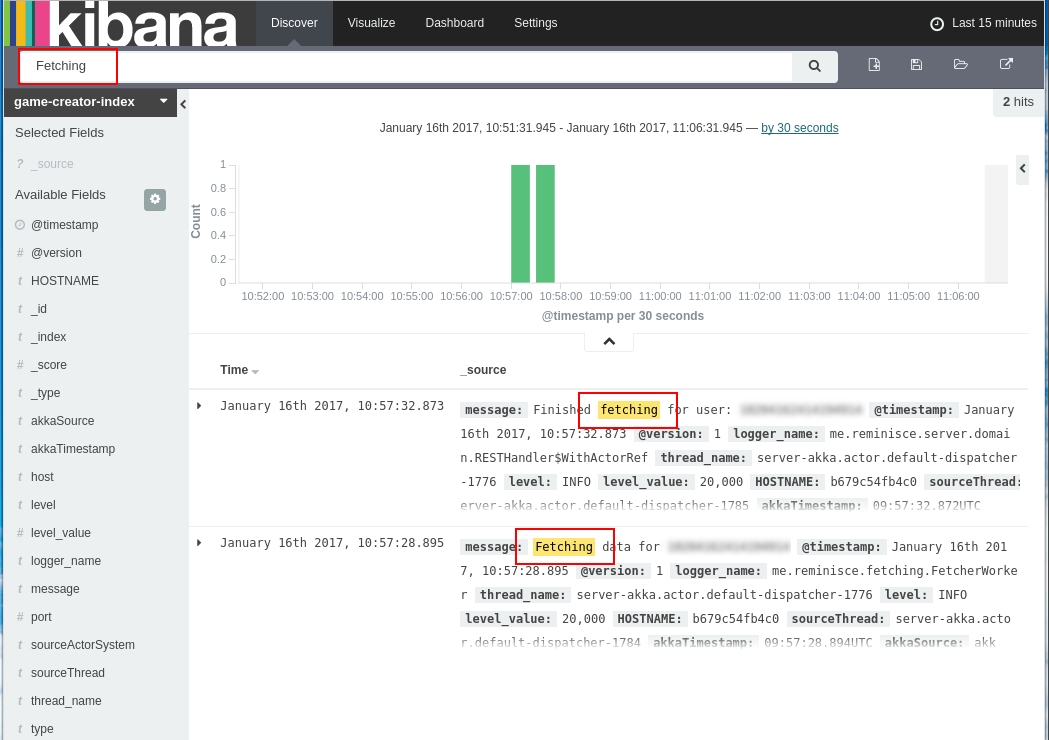
\includegraphics[width=6in]{images/kibana.png}}
\caption{Kibana Logs Interface}
\label{fig:kibana}
\end{figure}


\section{Stats module}\label{sec:stats}
The statistics module developed previously helped a lot in collecting data about the success rate of the user. However it had a major design flow which made the preprocessing step a potential stability threat. In short, the older the inserted game was, the more daily statistics had to be generated which could lead to resource starvation rather quickly (which simply means the module would crash or potentially worse, the whole server could stop). While all this preprocessing seemed like a good idea, we realized it was not necessary and decided to help with the simplification of the module's architecture.
\subsection{Collections and features}
The \textbf{cacheCollection} was replaced by a \textbf{statsCollection} which simply contains, for each day we have data about, the following information (called a 'daily statistic' later):
\begin{enumerate}
	\item \textbf{date} that day's date
	\item \textbf{amount} the number of games played
	\item \textbf{win} the number of wins
	\item \textbf{tie} the number of ties
	\item \textbf{loss} the number of losses
	\item \textbf{question breakdown} details for each question type containing the following:
	\begin{enumerate}
		\item \textbf{amount} number of those questions
		\item \textbf{correct} number of correct answer
		\item \textbf{wrong} number of wrong answers
		\item \textbf{avoid} number of avoided questions (non answered and not blocked by the other player)
		\item \textbf{time spent} total time spent on this type of question (in milliseconds)
	\end{enumerate}
\end{enumerate}
Aggregating by weeks months or years is then only a matter of performing some sums and can be done by the person requesting the data. If those aggregates were to become used a lot we could simply add their computation back into the new simpler architecture. The reason for their removal is that it was easier to remove them to sanitize the design of this module and then add them back into it\\
Obtaining data from the module is done in the same way as before: by issuing an HTTP GET request to the module. The parameters of the request however have changed. We only need to specify a starting and ending day and a limit. The module will then answer with a daily statistic for each day in the interval for which we have information (but not a larger number of them than the specified limit). If no date is provided for the start date we simply use the beginning of time and if no end date is specified we use today as an end date. The limit parameter was introduced to be able to request statistics about the last $n$ days a user used the application instead of using dates.\\
This modules uses logging the same way the Game Creator module does: it writes to a file which is then collected by Logstash.

\section{Summary}
The final architecture is then composed of the following components (see figure \ref{fig:architecture}):
\begin{itemize}
	\item \textbf{NginX proxy} in front of everything, responsible for dispatching the requests
	\item \textbf{Reminisce.me} the application itself, serving the user interface
	\item \textbf{Game Creator} the module responsible for serving questions to the application
	\item \textbf{Stats} the statistics module, compiling data about the success rate of users
	\item \textbf{Kibana, ElasticSearch, Logstash} the logging stack which helps monitoring everything
\end{itemize}
\begin{figure}
\centering
{\includegraphics[width=6in]{images/architecture.png}}
\caption{The whole architecture}
\label{fig:architecture}
\end{figure}